\documentclass[letter]{book}
\usepackage[
	urlcolor = blue,
	colorlinks = true,
	citecolor = black,
	linkcolor = black]{hyperref}
\usepackage{graphicx}
\usepackage{xltxtra}
\usepackage{fancyhdr}
\usepackage{booktabs}
\usepackage{indentfirst}
\usepackage{framed,color}
\usepackage{fancyvrb}
\usepackage{xcolor}
\usepackage{tikz}
\usepackage[framemethod=tikz]{mdframed}
\usepackage{caption}
\usepackage{pdfpages}
\usepackage{wrapfig}
\usepackage{perpage}
\usepackage{longtable}

\definecolor{shadecolor}{gray}{1.00}

\setromanfont{Hoefler Text}

\setmonofont[Scale=.85]{AndaleMono}

\settowidth{\parindent}{\qquad}

\title{The Riak Docs}
\author{Basho Technologies}

\makeatletter
\let\savedauthor=\@author
\let\savedtitle=\@title
\def\imgwidth{.6\linewidth}
\def\maxwidth{\ifdim\Gin@nat@width>\imgwidth\imgwidth
\else\Gin@nat@width\fi}
\makeatother

\title{\textbf{\savedtitle}}
\def\w3cdtfymd{1.4.9 \the\year-\ifnum\month<10 0\fi\the\month-\ifnum\day<10 0\fi\the\day}
\date{\w3cdtfymd}
\renewcommand{\thefootnote}{\fnsymbol{footnote}}

\makeatletter

  \setlength\headheight{12\p@}
  \setlength\headsep   {.25in}
  \setlength\topskip   {10\p@}
  \setlength\footskip{.35in}
  \setlength\textwidth{400\p@}
  
  \setlength\@tempdima{\paperheight}
  \addtolength\@tempdima{-2in}
  \divide\@tempdima\baselineskip
  \@tempcnta=\@tempdima
  \setlength\textheight{\@tempcnta\baselineskip}
  \addtolength\textheight{\topskip}
  
  \setlength\@tempdima        {\paperwidth}
  \addtolength\@tempdima      {-\textwidth}
  \setlength\oddsidemargin    {\paperwidth}
  \addtolength\oddsidemargin  {-2.35in}
  \addtolength\oddsidemargin  {-\textwidth}
  \setlength\marginparwidth   {0pt}
  \@settopoint\oddsidemargin
  \@settopoint\marginparwidth
  \setlength\evensidemargin  {\paperwidth}
  \addtolength\evensidemargin{-2.35in}
  \addtolength\evensidemargin{-\textwidth}
  \@settopoint\evensidemargin
  
  \setlength\topmargin{\paperheight}
  \addtolength\topmargin{-2in}
  \addtolength\topmargin{-\headheight}
  \addtolength\topmargin{-\headsep}
  \addtolength\topmargin{-\textheight}
  \addtolength\topmargin{-\footskip}
  \addtolength\topmargin{-.5\topmargin}
  \@settopoint\topmargin
\makeatother

\fancypagestyle{plain}{\fancyhf{}\fancyfoot[LE,RO]{\footnotesize\textbf\thepage}}
\pagestyle{plain}

\renewcommand{\headrulewidth}{0pt}
\renewcommand{\footrulewidth}{0pt}

\newcounter{img}[chapter]
\renewcommand{\theimg}{\thechapter.\arabic{img}}
\newcommand{\img}[2]{\begin{figure}[ht!]
	\refstepcounter{img}
	\label{img:\theimg}
  \centering\includegraphics[width=\maxwidth]{figures/#1.png}
  \textbf{\caption{#2}}
\end{figure}}

\newcounter{tab}[chapter]
\renewcommand{\thetab}{\thechapter.\arabic{tab}}

\newcommand{\prechap}{Chapter }
\newcommand{\postchap}{}
\newcommand{\presect}{Section }
\newcommand{\postsect}{}
\renewcommand{\chaptermark}[1]{\markboth{\textbf{\prechap \thechapter \postchap}\hspace*{1ex}#1}{}}
% \renewcommand{\sectionmark}[1]{\markright{\textbf{\presect \thesection \postsect}\hspace*{1ex}#1}}
\newcommand{\chap}[1]{\newpage\thispagestyle{empty}\chapter{#1}\label{chap:\thechapter}}
\newcommand{\chapref}[1]{\hyperref[chap:#1]{\prechap #1\postchap}}
\newcommand{\imgref}[1]{\hyperref[img:#1]{Figure #1}}
\newcommand{\tabref}[1]{\hyperref[tab:#1]{Table #1}}
\newcommand{\e}[1]{$ \times 10^{#1}$}
\renewcommand{\contentsname}{Contents}
\renewcommand{\figurename}{Figure }
\renewcommand{\tablename}{Table }

\makeatletter
\def\@makechapterhead#1{%
  \vspace*{50p@}%
  {\parindent \z@ \raggedright \normalfont
    \ifnum \c@secnumdepth >\m@ne
      \if@mainmatter
        \huge\bfseries \prechap \thechapter \postchap
        \par\nobreak
        \vskip 20\p@
      \fi
    \fi
    \interlinepenalty\@M
    \Huge \bfseries #1\par\nobreak
    \vskip 40\p@
  }}
\makeatother

\DefineShortVerb[commandchars=\\\{\}]{\|}
\DefineVerbatimEnvironment{Highlighting}{Verbatim}{commandchars=\\\{\},fontsize=\footnotesize}
\newenvironment{Shaded}{}{}
\newcommand{\KeywordTok}[1]{\textcolor[rgb]{0.00,0.44,0.13}{\textbf{{#1}}}}
\newcommand{\DataTypeTok}[1]{\textcolor[rgb]{0.56,0.13,0.00}{{#1}}}
\newcommand{\DecValTok}[1]{\textcolor[rgb]{0.25,0.63,0.44}{{#1}}}
\newcommand{\BaseNTok}[1]{\textcolor[rgb]{0.25,0.63,0.44}{{#1}}}
\newcommand{\FloatTok}[1]{\textcolor[rgb]{0.25,0.63,0.44}{{#1}}}
\newcommand{\CharTok}[1]{\textcolor[rgb]{0.25,0.44,0.63}{{#1}}}
\newcommand{\StringTok}[1]{\textcolor[rgb]{0.25,0.44,0.63}{{#1}}}
\newcommand{\CommentTok}[1]{\textcolor[rgb]{0.38,0.63,0.69}{\textit{{#1}}}}
\newcommand{\OtherTok}[1]{\textcolor[rgb]{0.00,0.44,0.13}{{#1}}}
\newcommand{\AlertTok}[1]{\textcolor[rgb]{1.00,0.00,0.00}{\textbf{{#1}}}}
\newcommand{\FunctionTok}[1]{\textcolor[rgb]{0.02,0.16,0.49}{{#1}}}
\newcommand{\RegionMarkerTok}[1]{{#1}}
\newcommand{\ErrorTok}[1]{\textcolor[rgb]{1.00,0.00,0.00}{\textbf{{#1}}}}
\newcommand{\NormalTok}[1]{{#1}}
% \ifxetex
%   \usepackage[setpagesize=false, % page size defined by xetex
%               unicode=false, % unicode breaks when used with xetex
%               xetex,
%               colorlinks=true,
%               linkcolor=blue]{hyperref}
% \else
%   \usepackage[unicode=true,
%               colorlinks=true,
%               linkcolor=blue]{hyperref}
% \fi
\hypersetup{breaklinks=true, pdfborder={0 0 0}}
\setlength{\parindent}{0pt}
\setlength{\parskip}{6pt plus 2pt minus 1pt}
\setlength{\emergencystretch}{3em}  % prevent overfull lines
\setcounter{secnumdepth}{0}

% \EndDefineVerbatimEnvironment{Highlighting}

\mdfdefinestyle{AsideFrame}{%
    outerlinewidth=0pt,
    leftline=false,
    rightline=false,
    topline=false,
    bottomline=false,
    roundcorner=6pt,
    innerbottommargin=0.6\baselineskip,
    innertopmargin=0.6\baselineskip,
    skipabove=7pt,
    skipbelow=7pt,
    % font=\Huge,
    backgroundcolor=gray!20
    % splittopskip=0.5\baselineskip,
    % frametitleaboveskip=\baselineskip% \baselineskip distance from top rule
    }

% \newenvironment{aside}[1][]
%   {\begin{mdframed}[style=0,%
%       leftline=false,rightline=false,leftmargin=2em,rightmargin=2em,%
%       innerleftmargin=18pt,innerrightmargin=18pt,linewidth=0pt,%
%       innerbottommargin=0.6\baselineskip,innertopmargin=0.6\baselineskip,%
%       roundcorner=10pt,backgroundcolor=gray!20,%
%       skipabove=7pt,skipbelow=7pt,font=\small,#1]\small}
%   {\end{mdframed}}

\newenvironment{aside}[1][]
  {\begin{mdframed}[style=AsideFrame,font=\small,#1]\small}
  {\end{mdframed}}


\linespread{1.3}

\begin{document}
\frontmatter
\maketitle
\vspace*{2.5in}
\begin{center}
    This book is licensed under the Creative Commons Attribution-Non Commercial-Share Alike 3.0 license.

    Body typeface is Crimson.
\end{center}
\setcounter{tocdepth}{4}
\tableofcontents\newpage\thispagestyle{empty}

\renewcommand{\thefootnote}{\arabic{footnote}}

\mainmatter
\fancyhf{}
\fancyhead[LE]{{\small\leftmark}}
\fancyhead[RO]{{\small\rightmark}}
\fancyhead[RE,LO]{{\small\savedauthor\hspace*{1ex}\textbf{\savedtitle}}}
\fancyfoot[LE,RO]{\small\textbf\thepage}
\pagestyle{fancy}

\section{What is Riak?}\label{what-is-riak}

Riak is a distributed database designed to deliver maximum data availability by distributing data across multiple servers. As long as your client can reach \emph{one} Riak server, it should be able to write data. In most failure scenarios, the data you want to read should be available, although it may not be the most up-to-date version of that data.

This fundamental tradeoff---high availability in exchange for possibly outdated information---informs the key architectural decisions behind Riak. This idea of “eventual consistency” is a common one in distributed systems, with DNS and web caches as two notable examples.

\subsection{Basho's goals for Riak}\label{bashos-goals-for-riak}

\begin{longtable}[c]{@{}ll@{}}
\toprule\addlinespace
Goal & Description
\\\addlinespace
\midrule\endhead
\textbf{Availability} & Riak writes to and reads from multiple servers to offer data availability even when hardware or the network itself are experiencing failure conditions
\\\addlinespace
\textbf{Operational simplicity} & Easily add new machines to your Riak cluster without incurring a larger operational burden
\\\addlinespace
\textbf{Scalability} & Riak automatically distributes data around the cluster and yields a near-linear performance increase as you add capacity
\\\addlinespace
\textbf{Masterless} & Your requests are not held hostage to a specific server in the cluster that may or may not be available
\\\addlinespace
\bottomrule
\end{longtable}

\subsection{When Riak makes sense}\label{when-riak-makes-sense}

If your data does not fit on a single server and demands a distributed database architecture, then you should absolutely take a close look at Riak as a potential solution to your data availability issues. Getting distributed databases right is \textbf{very} difficult, and Riak was built to address data availability issues with as few trade-offs and downsides as possible.

In essence, Riak's focus on availability makes it a good fit whenever downtime is unacceptable. No one can promise 100\% uptime, but Riak is designed to survive network partitions and hardware failures that would significantly disrupt most databases.

A less-heralded feature of Riak is its predictable latency. Because its fundamental operations---read, write, and delete---do not involve complex data joins or locks, it services those requests promptly. Thanks to this capability Riak is often selected as a data storage backend for other data management software from a variety of paradigms.

\subsection{When Riak is Less of a Good Fit}\label{when-riak-is-less-of-a-good-fit}

Basho recommends that you run no fewer than 5 data servers in a cluster. This means that Riak can be overkill for small databases. If you're not already sure that you will need a distributed database, there's a good chance that you won't need Riak.

Nonetheless, if explosive growth is a possibility, you are always highly advised to prepare for that in advance. Scaling at Internet speeds is sometimes compared to overhauling an airplane mid-flight. If you feel that such a transition might be necessary in the future, then you might want to consider Riak.

Riak's simple data model, consisting of keys and values as its atomic elements, means that your data must be denormalized if your system is to be reasonably performant. For most applications this is not a serious hurdle. But if your data simply cannot be effectively managed as keys and values Riak will most likely not be the best fit for you.

On a related note: while Riak offers ways to find values that match certain criteria, if your application demands a high query load by any means other than the keys---e.g.~SQL-style \texttt{SELECT * FROM table} operations---Riak will not be as efficient as other databases. If you wish to compare Riak with other data technologies, Basho offers a tool called \textbf{basho\_bench} to help measure its performance so that you can decide whether the availability and operational benefits of Riak outweigh its disadvantages.

\section{How Does a Riak Cluster Work?}\label{how-does-a-riak-cluster-work}

\subsection{What is a Riak Node?}\label{what-is-a-riak-node}

A Riak node is not quite the same as a server, but in a production environment the two should be equivalent. A developer may run multiple nodes on a single laptop, but this would never be advisable in a real production cluster.

Each node in a Riak cluster is equivalent, containing a complete, independent copy of the whole Riak package. There is no “master.” No node has more responsibilities than others, and no node has special tasks not performed by other nodes. This uniformity provides the basis for Riak's fault tolerance and scalability.

Each node is responsible for multiple data partitions as discussed below.

\subsection{Riak Automatically Re-Distributes Data When Capacity is Added}\label{riak-automatically-re-distributes-data-when-capacity-is-added}

When you add (or remove) machines, data is rebalanced automatically with no downtime. New machines claim data until ownership is equally spread around the cluster, with the resulting cluster status updates shared to every node via a gossip protocol and used to route requests. This is what makes it possible for any node in the cluster to receive requests. The end result is that developers don't need to deal with the underlying complexity of where data lives.

\subsection{Consistent Hashing}\label{consistent-hashing}

Data is distributed across nodes using consistent hashing. Consistent hashing ensures that data is evenly distributed around the cluster and makes possible the automatic redistribution of data as the cluster scales.

How does consistent hashing work? Riak stores data using a simple key/value scheme. These keys are associated with a namespace called a \textbf{bucket}. When you perform key/value operations in Riak, the bucket and key combination is hashed. The resulting hash maps onto a 160-bit integer space. You can think of this integer space as a ring used to determine what data to put on which physical machines.

How is this determination made? Riak divides the integer space into equally-sized partitions. Each partition owns a range of values on the ring, and is responsible for all buckets and keys that, when hashed, fall into that range. Each partition is managed by a process called a virtual node (or \textbf{vnode}*). Physical machines evenly divide responsibility for vnodes. Let's say that you have a 4-node cluster with 32 partitions managed by 32 vnode processes. Each of the four physical machines claim eight vnodes (as illustrated below). Each physical machine thus becomes responsible for all keys represented by its eight vnodes.

\begin{figure}[htbp]
\centering
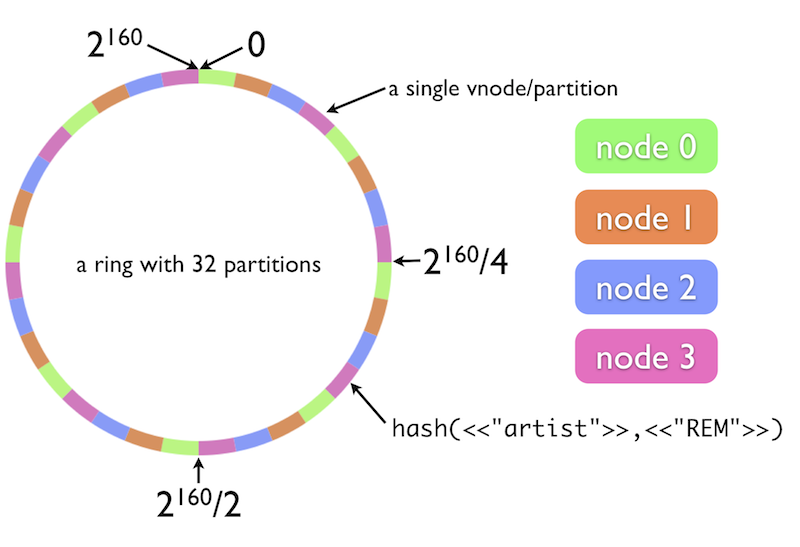
\includegraphics{../source/images/riak-ring.png}
\caption{A Riak Ring}
\end{figure}

\subsection{Intelligent Replication}\label{intelligent-replication}

Riak's replication scheme ensures that you can still read, write, and update data if nodes go down. Riak allows you to set a replication variable, \emph{n}. An \emph{n} value of 3 (the default) means that each object is replicated 3 times. When an object's key is mapped onto a given partition, Riak won't stop there: it will automatically replicate the data onto the next two partitions as well.

\begin{figure}[htbp]
\centering
\includegraphics{../source/images/riak-data-distribution.png}
\caption{A Riak Ring}
\end{figure}

\section{When Things Go Wrong}\label{when-things-go-wrong}

Riak retains fault tolerance, data integrity, and availability even in failure conditions such as hardware failure and network partitions. Riak has a number of means of addressing these scenarios and other bumps in the road, like version conflicts in data.

\subsection{Hinted Handoff}\label{hinted-handoff}

Hinted handoff enables Riak to handle node failure. If a node goes down, a neighboring node will take over its storage operations. When the failed node returns, the updates received by the neighboring node are handed back to it. This ensures availability for writes and updates and happens automatically, minimizing the operational burden of failure conditions.

\subsection{Version Conflicts}\label{version-conflicts}

In any system that replicates data, conflicts can arise, for example when two clients update the same object at the exact same time or when not all updates have yet reached hardware that is experiencing lag. Furthermore, in Riak, replicas are “eventually consistent,” meaning that while data is always available, not all replicas may have the most recent update at the exact same time, causing brief periods---generally on the order of milliseconds---of inconsistency while all state changes are synchronized.

How is this divergence addressed? When you make a read request, Riak looks up all replicas for that object. By default, Riak will return the most recently updated version, determined by looking at the object's vector clock. Vector clocks are metadata attached to each replica when it is created. They are extended each time a replica is updated to keep track of versions. You can also allow clients to resolve conflicts themselves if that is a better fit for your use case.

\subsection{Read Repair}\label{read-repair}

When an outdated replica is returned as part of a read request, Riak will automatically update the out-of-sync replica to make it consistent. Read repair, a self-healing property of the database, will even update a replica that returns a \texttt{not\_found} in the event that a node loses the data due to physical failure.

\subsection{Reading and Writing Data in Failure Conditions}\label{reading-and-writing-data-in-failure-conditions}

In Riak, you can set an \emph{r} value for reads and a \emph{w} value for writes. These values give you control over how many replicas must respond to a request for it to succeed. Let's say that you have an \emph{n} value of 3, but one of the physical nodes responsible for a replica is down. With an r=2 setting, only 2 replicas must return results for read to be deemed successful. This allows Riak to provide read availability even when nodes are down or laggy. The same applies for the \emph{w} in writes. If this value is not specified, Riak defaults to \textbf{quorum}, according to which the majority of nodes must respond. There is more on {[}{[}Replication Properties{]}{]} elsewhere in the documentation.

This is intended to be a brief, objective and technical comparison of Riak and Cassandra. The Cassandra version described is 1.2.x. The Riak version described is Riak 1.2.x. If you feel this comparison is unfaithful at all for whatever reason, please \href{https://github.com/basho/basho_docs/issues/new}{fix it} or send an email to \textbf{docs@basho.com}.

\section{At A Very High Level}\label{at-a-very-high-level}

\begin{itemize}
\itemsep1pt\parskip0pt\parsep0pt
\item
  Both Riak and Cassandra are Apache 2.0 licensed databases based on Amazon's Dynamo paper.
\item
  Riak is a faithful implementation of Dynamo, with the addition of functionality like links, MapReduce, indexes, full-text Search. Cassandra departs from the Dynamo paper slightly by omitting vector clocks and moving from partition-based consistent hashing to key ranges, while adding functionality like order-preserving partitioners and range queries.
\item
  Riak is written primarily in Erlang with some bits in C. Cassandra is written in Java.
\end{itemize}

\section{Feature/Capability Comparison}\label{featurecapability-comparison}

The table below gives a high level comparison of Riak and Cassandra features/capabilities. To keep this page relevant in the face of rapid development on both sides, low level details are found in links to Riak and Cassandra online documentation.

Feature/Capability

Riak

Cassandra

Data Model

Riak stores key/value pairs in a higher level namespace called a bucket.

{[}{[}Buckets, Keys, and Values\textbar{}Concepts\#Buckets-Keys-and-Values{]}{]}

Cassandra's data model resembles column storage, and consists of Keyspaces, Column Families, and several other parameters.

{[}{[}Cassandra Data Model\textbar{}http://www.datastax.com/docs/0.7/data\_model/index{]}{]}

Storage Model

Riak has a modular, extensible local storage system which lets you plug-in a backend store of your choice to suit your use case. The default backend is Bitcask.

{[}{[}Riak Supported Storage Backends\textbar{}Choosing a Backend{]}{]}

\begin{shaded}\begin{verbatim}
    You can also write you own storage backend for Riak using our [[backend API|Backend API]].
 </td>
    <td> Cassandra's write path starts with a write to a commit log followed by a subsequent write to an in-memory structure called a memtable. Writes are then batched to a persistent table structure called a sorted string table (SST).
        <ul>
          <li><a href="http://wiki.apache.org/cassandra/ArchitectureCommitLog">Commit Log</a></li>
        <li><a href="http://wiki.apache.org/cassandra/MemtableSSTable">Memtable</a></li>
        <li><a href="http://wiki.apache.org/cassandra/ArchitectureSSTable">SSTable Overview</a></li>
        <li><a href="http://www.datastax.com/docs/1.1/dml/about_writes">About Writes</a></li>
        <li><a href="http://www.datastax.com/docs/1.1/dml/about_reads">About Reads</a></li>
        </ul>
    </td>
</tr>
<tr>
    <td>Data Access and APIs</td>
    <td>Riak offers two primary interfaces (in addition to raw Erlang access):
		<ul>
		  <li>[[HTTP|HTTP API]]</li>
		<li>[[Protocol Buffers|PBC API]]</li>
		</ul>
		Riak Client libraries are wrappers around these APIs, and client support exists for dozens of languages. 
		<ul>
		  <li>[[Client Libraries]]</li>
		  <li>[[Community Projects]] </li>
		</ul>
		</td>
    <td>Cassandra provides various access methods including a Thrift API, CQL (Cassandra Query Language), and CLI. 
		<ul>
		  <li><a href="http://www.datastax.com/docs/1.1/dml/about_clients">Cassandra Client APIs</a></li>
		</ul>		
 </td>
</tr>
<tr>
    <td>Query Types and Query-ability</td>
    <td>There are currently four ways to query data in Riak
        <ul>
        <li>Primary key operations (GET, PUT, DELETE, UPDATE)</li>
        <li>[[MapReduce|Using MapReduce]]</li>
        <li>[[Using Secondary Indexes]]</li>
        <li>[[Using Search]]</li>
        </ul>

</td>
    <td>Cassandra offers various ways to query data:
            <ul>
            <li><a href="http://www.datastax.com/docs/0.7/data_model/keyspaces">Keyspaces</a></li>
            <li><a href="http://www.datastax.com/docs/0.7/data_model/cfs_as_indexes">Column Family Operations</a></li>
            <li><a href="http://www.datastax.com/docs/1.0/dml/using_cql">CQL</a></li>
            <li><a href="http://www.datastax.com/docs/0.7/data_model/secondary_indexes">Secondary Indexes</a></li>
            <li><a href="http://wiki.apache.org/cassandra/HadoopSupport#ClusterConfig">Hadoop Support</a></li>
        <ul>

</td>
</tr>
<tr>
    <td>Data Versioning and Consistency</td>
    <td> Riak uses a data structure called a vector clock to reason about causality and staleness of stored values. Vector clocks enable clients to always write to the database in exchange for consistency conflicts being resolved at read time by either application or client code. Vector clocks can be configured to store copies of a given datum based on size and age of said datum.   There is also an option to disable vector clocks and fall back to simple time-stamp based "last-write-wins".
        <ul>
          <li>[[Vector Clocks]]</li>
          <li>[[Why Vector Clocks Are Easy|http://basho.com/blog/technical/2010/01/29/why-vector-clocks-are-easy/]]</li>
          <li>[[Why Vector Clocks Are Hard|http://basho.com/blog/technical/2010/04/05/why-vector-clocks-are-hard/]]</li>
        </ul>
     </td>

    <td>Cassandra uses timestamps at the column family level to determine the most-recent value when doing read requests. There is no built-in way to do versioning of data.
        <ul>
          <li>[[About Read Consistency|http://www.datastax.com/docs/1.1/dml/data_consistency#about-read-consistency]]</li>
        </ul>
 </td>
</tr>
    </tr>
        <td>Concurrency</td>
        <td>In Riak, any node in the cluster can coordinate a read/write operation for any other node. Riak stresses availability for writes and reads, and puts the burden of resolution on the client at read time.
        </td>

        <td>All nodes in Cassandra are peers. A client read or write request can go to any node in the cluster. When a client connects to a node and issues a read or write request, that node serves as the coordinator for that particular client operation.
            <ul>
                <li>[[About Client Requests|http://www.datastax.com/docs/1.0/cluster_architecture/about_client_requests]]
            </ul>
     </td>
    </tr>
<tr>
    <td>Replication</td>
    <td>Riak's replication system is heavily influenced by the Dynamo Paper and Dr. Eric Brewer's CAP Theorem. Riak uses consistent hashing to replicate and distribute N copies of each value around a Riak cluster composed of any number of physical machines. Under the hood, Riak uses virtual nodes to handle the distribution and dynamic rebalancing of data, thus decoupling the data distribution from physical assets.
        <ul>
          <li>[[Replication]]</li>
          <li>[[Clustering|Concepts#Clustering]]</li>
        </ul>

        The Riak APIs expose tunable consistency and availability parameters that let you select which level configuration is best for your use case. Replication is configurable at the bucket level when first storing data in Riak. Subsequent reads and writes to that data can have request-level parameters.
            <ul>
                <li>[[Reading, Writing, and Updating Data|Concepts#Reading-Writing-and-Updating-Data]]</li>
            </ul>

 </td>
    <td>Replication in Cassandra starts when a user chooses a partitioner. Partitioners include Random Partitioner (which also relies on consistent hashing for data storage) and various Ordered Partitioner options. Under the hood, physical nodes are assigned tokens which determine a nodes's position on the ring and the range of data for which it's responsible.
        <ul>
          <li>[[Replication|http://www.datastax.com/docs/1.0/cluster_architecture/replication]]</li>
        </ul>

        Like in Riak, Cassandra lets developers configure the consistency and availability requirements at the request level via various APIs.
        <ul>
            <li><a href="http://www.datastax.com/docs/1.1/dml/data_consistency#tunable-consistency">Tunable Consistency</a>
        </ul>

 </td>
</tr>
<tr>
    <td>Scaling Out and In</td>
    <td>Riak allows you to elastically grow and shrink your cluster while evenly balancing the load on each machine. No node in Riak is special or has any particular role. In other words, all nodes are masterless. When you add a physical machine to Riak, the cluster is made aware of its membership via gossiping of ring state. Once it's a member of the ring, it's assigned an equal percentage of the partitions and subsequently takes ownership of the data belonging to those partitions. The process for removing a machine is the inverse of this. Riak also ships with a comprehensive suite of command line tools to help make node operations simple and straightforward.

<ul>
    <li>[[Adding and Removing Nodes]]</li>
    <li>[[Command Line Tools]]</li>
</ul>

    <td>Cassandra allows you to add new nodes dynamically with the exception of manually calculating a node's token (though users can elect to let Cassandra calculate this). It's recommended that you double the size of your cluster to add capacity. If this isn't feasible, you can elect to either add a number of nodes (which requires token recalculation for all existing nodes), or to add one node at a time, which means leaving the initial token blank and "will probably not result in a perfectly balanced ring but it will alleviate hot spots".
        <ul>
          <li>[[Adding Capacity to an Existing Cluster|http://www.datastax.com/docs/1.1/operations/cluster_management#adding-capacity-to-an-existing-cluster]]</li>
        </ul>
</td>
</tr>
<tr>
    <td>Multi-Datacenter Replication</td>

    <td>Riak features two distinct types of replication. Users can replicate to any number of nodes in one cluster (which is usually contained within one datacenter over a LAN) using the Apache 2.0 database. Riak Enterprise, Basho's commercial extension to Riak, is required for Multi-Datacenter deployments (meaning the ability to run active Riak clusters in N datacenters).

    <ul>
        <li><a href="http://basho.com/products/riak-enterprise/">Riak Enterprise</a></li>
    <ul>

    <td>Cassandra has the ability to spread nodes over multiple datacenters via various configuration parameters.
        <ul>
          <li>[[Multiple Datacenters|http://www.datastax.com/docs/1.1/initialize/cluster_init_multi_dc]]</li>
        </ul>

</td>
</tr>
<tr>
    <td>Graphical Monitoring/Admin Console</td>
    <td>Riak ships with Riak Control, an open source graphical console for monitoring and managing Riak clusters.
        <ul>
            <li>[[Riak Control]]</li>
            <li>[[Introducing Riak Control|http://basho.com/blog/technical/2012/02/22/Riak-Control/]]
        </ul>
</td>
    <td>Datastax distributes the DataStax OpsCenter, a graphical user interface for monitoring and administering Cassandra clusters. This includes a free version available for production use, as well as a for-pay version with additional features.
        <ul>
            <li>[[DataStax OpsCenter|http://www.datastax.com/products/opscenter]]</li>
        </ul>
 </td>
</tr>
\end{verbatim}\end{shaded}

This is intended to be a brief, objective and technical comparison of Riak and Couchbase (i.e.~Couchbase Server). The Couchbase version described is 2.0. The Riak version described is Riak 1.2.x. If you feel this comparison is unfaithful at all for whatever reason, please \href{https://github.com/basho/basho_docs/issues/new}{fix it} or send an email to \textbf{docs@basho.com}.

\section{At A Very High Level}\label{at-a-very-high-level-1}

\begin{itemize}
\itemsep1pt\parskip0pt\parsep0pt
\item
  Riak is Apache 2.0 licensed; According to Couchbase, they have two free versions: Couchbase open source is Apache 2.0 licensed; Couchbase Server Community Edition (free version) is licensed under a \href{http://www.couchbase.com/agreement/community}{community agreement}
\item
  Riak is written primarily in Erlang with some bits in C; Couchbase is written in Erlang and C/C++
\end{itemize}

Couchbase vs CouchDB

Keep in mind that Couchbase and CouchDB are two separate database projects. CouchDB is a document database providing replication, MapReduce and an HTTP API. Couchbase uses CouchDB as its backend, “wrapping” it with advanced features like caching, and is designed to be clustered.

Couchbase 2.0

As of the time of this writing, Couchbase 2.0 is still in developer preview, so some of these points may change between now and the final release. Caveat emptor

\section{Feature/Capability Comparison}\label{featurecapability-comparison-1}

The table below gives a high level comparison of Riak and Couchbase features/capabilities. To keep this page relevant in the face of rapid development on both sides, low level details are found in links to Riak and Couchbase online documentation.

\begin{shaded}\begin{verbatim}
    <th WIDTH="15%">Feature/Capability</th>
    <th WIDTH="42%">Riak</th>
    <th WIDTH="43%">Couchbase</th>
</tr>
<tr>
    <td>Data Model</td>
    <td>Riak stores key/value pairs in a higher level namespace called a bucket.
        <ul>
          <li>[[Buckets, Keys, and Values|Concepts#Buckets-Keys-and-Values]] </li>
        </ul>
    </td>
    <td>Couchbase is a JSON-based document datastore. Like other document datastores, records have no intrinsic relationships, and are stored in buckets. Value size is limited to 20Mbyte.
        <ul>
            <li>[[How Should I Store an Object?|http://www.couchbase.com/docs/couchbase-manual-2.0/couchbase-developing-bestpractices-objectstorage-how.html]]</li>
        </ul>
    </td>
</tr>
<tr>
    <td>Storage Model</td>
    <td>Riak has a modular, extensible local storage system which lets you plug-in a backend store of your choice to suit your use case. The default backend is Bitcask.
        <ul>
          <li>[[Riak Supported Storage Backends|Choosing a Backend]]</li>
        </ul>

    You can also write your own storage backend for Riak using our [[backend API|Backend API]].
 </td>
    <td>Couchbase 2.0 is largely memory-based, asynchronously persisting data using a CouchDB fork and C library "couchstore" (prior versions of Couchbase use the SQLite storage engine).
        <ul>
        <li>[[Persistence|http://www.couchbase.com/docs/couchbase-manual-2.0/couchbase-architecture-persistencedesign.html]]</li>
        <li>[[Couchbase File Format|https://github.com/couchbaselabs/couchstore/wiki/Format]]</li>
        </ul>
    </td>
</tr>
<tr>
    <td>Data Access and APIs</td>
    <td>Riak offers two primary interfaces (in addition to raw Erlang access):
		<ul>
		<li>[[HTTP|HTTP API]]</li>
		<li>[[Protocol Buffers|PBC API]]</li>
		</ul>
		Riak Client libraries are wrappers around these APIs, and client support exists for dozens of languages. 
		<ul>
		<li>[[Client Libraries]]</li>
		<li>[[Community Projects]]</li>
		</ul>
		</td>
    <td>Couchbase provides drivers in several languages to access data through its binary memcached protocol. Couchbase also provides a REST API to monitor and manage a cluster (though it is not used to directly manage stored data).
        <ul>
            <li>[[Client Interface|http://www.couchbase.com/docs/couchbase-manual-2.0/couchbase-introduction-architecture-clientinterface.html]]</li>
            <li>[[Client-Libraries|http://www.couchbase.com/develop]]</li>
            <li>[[Management REST API|http://www.couchbase.com/docs/couchbase-manual-2.0/couchbase-admin-restapi.html]]</li>
        </ul>
 </td>
</tr>
<tr>
    <td>Query Types and Query-ability</td>
    <td>There are currently four ways to query data in Riak
        <ul>
        <li>Primary key operations (GET, PUT, DELETE, UPDATE)</li>
        <li>[[Using MapReduce]]</li>
        <li>[[Using Secondary Indexes]]</li>
        <li>[[Using Search]]</li>
        </ul>
</td>
    <td>Couchbase also provides four query options
        <ul>
        <li>[[ID lookups|http://www.couchbase.com/docs/couchbase-manual-2.0/couchbase-developing-bestpractices-multiget.html]]</li>
        <li>[[MapReduce Views|http://www.couchbase.com/docs/couchbase-manual-2.0/couchbase-views-basics.html]]</li>
        <li>[[UnQL|http://www.couchbase.com/press-releases/unql-query-language]]</li>
        </ul>
        Hadoop support is also possible through a plugin that streams data to a Hadoop Distributed File System (HDFS) or Hive for processing.
        <ul>
        <li>[[Hadoop Connector|http://www.couchbase.com/develop/connectors/hadoop]]</li>
        <ul>
</td>
</tr>
<tr>
    <td>Data Versioning and Consistency</td>
    <td> Riak uses a data structure called a vector clock to reason about causality and staleness of stored values. Vector clocks enable clients to always write to the database in exchange for consistency conflicts being resolved at read time by either application or client code. Vector clocks can be configured to store copies of a given datum based on size and age of said datum.   There is also an option to disable vector clocks and fall back to simple time-stamp based "last-write-wins".
        <ul>
          <li>[[Vector Clocks]]</li>
          <li>[[Why Vector Clocks Are Easy|http://basho.com/blog/technical/2010/01/29/why-vector-clocks-are-easy/]]</li>
          <li>[[Why Vector Clocks Are Hard|http://basho.com/blog/technical/2010/04/05/why-vector-clocks-are-hard/]]</li>
        </ul>
     </td>

    <td>Couchbase is strongly consistent within a datacenter, replicating data between nodes in a cluster for failover. Inter-datacenter replication follows an eventually consistent CouchDB replication model.

        Via CouchDB, documents are internally revisioned (stored in a "_rev" value). However, prior revisions will be removed on a file compaction operation, making them unreliable.

    <ul>
    <li>[[Couchbase Architecture|http://www.couchbase.com/docs/couchbase-manual-2.0/couchbase-architecture.html]]</li>
    <li>[[Internal Version Field|http://www.couchbase.com/docs/couchbase-manual-2.0/couchbase-views-datastore-fields.html]]</li>
    </ul>
</tr>
    <td>Concurrency</td>
    <td> In Riak, any node in the cluster can coordinate a read/write operation for any other node. Riak stresses availability for writes and reads, and puts the burden of resolution on the client at read time.
     </td>

    <td>Couchbase claims to be ACID-compliant on a per-item basis, but has no multi-operation transactions. Couchbase clients connect to a server list (or via a proxy) where keys are sharded across the nodes. Couchbase nodes inherit memcached's default (and recommended) connection limit of 10k.

    <ul>
    <li>[[Transaction and concurrency|http://www.couchbase.com/forums/thread/transaction-and-concurency]]</li>
    <li>[[Cluster Design|http://www.couchbase.com/docs/couchbase-manual-2.0/couchbase-architecture-clusterdesign.html]]</li>
    <li>[[Client-side Proxy|http://www.couchbase.com/docs/couchbase-manual-2.0/couchbase-deployment-standaloneproxy.html]]</li>
    </ul>

 </td>
</tr>
<tr>
    <td>Replication</td>
    <td>Riak's replication system is heavily influenced by the Dynamo Paper and Dr. Eric Brewer's CAP Theorem. Riak uses consistent hashing to replicate and distribute N copies of each value around a Riak cluster composed of any number of physical machines. Under the hood, Riak uses virtual nodes to handle the distribution and dynamic rebalancing of data, thus decoupling the data distribution from physical assets.
        <ul>
          <li>[[Replication]]</li>
          <li>[[Clustering|Concepts#Clustering]]</li>
        </ul>

        The Riak APIs expose tunable consistency and availability parameters that let you select which level configuration is best for your use case. Replication is configurable at the bucket level when first storing data in Riak. Subsequent reads and writes to that data can have request-level parameters.
            <ul>
                <li>[[Reading, Writing, and Updating Data|Concepts#Reading-Writing-and-Updating-Data]]</li>
            </ul>

 </td>
 <td>Couchbase supports two types of replication.  For intra-datacenter clusters, Couchbase uses membase-style replication, which favors immediate consistency in the face of a network partition.  For multi-datacenter deployments, CouchDB's master-master replication is used.

        <ul>
        <li>[[CouchDB Replication|http://wiki.apache.org/couchdb/Replication]]</li>
        <li>[[Memcache Tap|http://code.google.com/p/memcached/wiki/Tap]]</li>
        <li>[[CouchDB, Couchbase, Membase|http://www.infoq.com/news/2012/05/couchdb-vs-couchbase-membase]]</li>

        </ul>
 </td>
</tr>
<tr>
    <td>Scaling Out and In</td>
    <td>Riak allows you to elastically grow and shrink your cluster while evenly balancing the load on each machine. No node in Riak is special or has any particular role. In other words, all nodes are masterless. When you add a physical machine to Riak, the cluster is made aware of its membership via gossiping of ring state. Once it's a member of the ring, it's assigned an equal percentage of the partitions and subsequently takes ownership of the data belonging to those partitions. The process for removing a machine is the inverse of this. Riak also ships with a comprehensive suite of command line tools to help make node operations simple and straightforward.

<ul>
    <li>[[Adding and Removing Nodes]]</li>
    <li>[[Command Line Tools]]</li>
</ul>
    </td>
    <td>Couchbase scales elastically by auto-sharding. They can be rebalanced to grow or shrink through the administrative interface.

    <ul>
    <li>[[Rebalancing|http://www.couchbase.com/docs/couchbase-manual-2.0/couchbase-admin-tasks-addremove.html]]</li>
    <li>[[Clone to Grow with Auto Sharding|http://www.couchbase.com/couchbase-server/features#clone_to_grow]]</li>
    </ul>
</td>
</tr>
<tr>
    <td>Multi-Datacenter Replication and Awareness</td>

    <td>Riak features two distinct types of replication. Users can replicate to any number of nodes in one cluster (which is usually contained within one datacenter over a LAN) using the Apache 2.0 licensed database. Riak Enterprise, Basho's commercial extension to Riak, is required for Multi-Datacenter deployments (meaning the ability to run active Riak clusters in N datacenters).

    <ul>
        <li><a href="http://basho.com/products/riak-enterprise/">Riak Enterprise</a></li>
    </ul>

    </td>
    <td>Couchbase 2.0 supports cross-datacenter replication (XDCR).

    <ul>
    <li>[[Stabilizing Couchbase Server 2.0|http://blog.couchbase.com/stabilizing-couchbase-server-2-dot-0]]</li>
    </ul>
</td>
</tr>
<tr>
    <td>Graphical Monitoring/Admin Console</td>
    <td>Riak ships with Riak Control, an open source graphical console for monitoring and managing Riak clusters.
        <ul>
            <li>[[Riak Control]]</li>
            <li>[[Introducing Riak Control|http://basho.com/blog/technical/2012/02/22/Riak-Control/]]
        </ul>
</td>
    <td>Couchbase provides a web-based monitoring/admin console.
        <ul>
            <li>[[Admin Wed Console|http://www.couchbase.com/docs/couchbase-manual-2.0/couchbase-admin-web-console.html]]</li>
            <li>[[Monitoring Couchbase|http://www.couchbase.com/docs/couchbase-manual-2.0/couchbase-monitoring.html]]</li>
        </ul>

 </td>
</tr>
\end{verbatim}\end{shaded}

This is intended to be a brief, objective and technical comparison of Riak and CouchDB. The CouchDB version described is 1.2.x. The Riak version described is Riak 1.2.x. If you feel this comparison is unfaithful at all for whatever reason, please \href{https://github.com/basho/basho_docs/issues/new}{fix it} or send an email to \textbf{docs@basho.com}.

\section{At A Very High Level}\label{at-a-very-high-level-2}

\begin{itemize}
\itemsep1pt\parskip0pt\parsep0pt
\item
  Riak and CouchDB are both Apache 2.0 licensed
\item
  Riak is written primarily in Erlang with some bits in C; CouchDB is written in Erlang
\end{itemize}

\section{Feature/Capability Comparison}\label{featurecapability-comparison-2}

The table below gives a high level comparison of Riak and CouchDB features/capabilities. To keep this page relevant in the face of rapid development on both sides, low level details are found in links to Riak and CouchDB online documentation.

\begin{shaded}\begin{verbatim}
    <th WIDTH="15%">Feature/Capability</th>
    <th WIDTH="42%">Riak</th>
    <th WIDTH="43%">CouchDB</th>
</tr>
<tr>
    <td>Data Model</td>
    <td>Riak stores key/value pairs in a higher level namespace called a bucket.
        <ul>
          <li>[[Buckets, Keys, and Values|Concepts#Buckets-Keys-and-Values]] </li>
        </ul>
    </td>
    <td>CouchDB's data format is JSON stored as documents (self-contained records with no intrinsic relationships), grouped into "database" namespaces.
        <ul>
            <li>[[Document API|http://wiki.apache.org/couchdb/HTTP_Document_API]]</li>
        </ul>
    </td>
</tr>
<tr>
    <td>Storage Model</td>
    <td>Riak has a modular, extensible local storage system which lets you plug-in a backend store of your choice to suit your use case. The default backend is Bitcask.
        <ul>
          <li>[[Riak Supported Storage Backends|Choosing a Backend]]</li>
        </ul>

    You can also write your own storage backend for Riak using our [[backend API|Backend API]].
 </td>
    <td>CouchDB stores data to disk by "append-only" files. As the files continue to grow, they require occasional compaction.
        <ul>
         <li>[[Indexes and File|http://guide.couchdb.org/draft/btree.html]]</li>
        </ul>
    </td>
</tr>
<tr>
    <td>Data Access and APIs</td>
    <td>Riak offers two primary interfaces (in addition to raw Erlang access):
		<ul>
		  <li>[[HTTP|HTTP API]]</li>
		<li>[[Protocol Buffers|PBC API]]</li>
		</ul>
		Riak Client libraries are wrappers around these APIs, and client support exists for dozens of languages. 
		<ul>
		<li>[[Client Libraries]]</li>
		<li>[[Community Projects]]</li>
		</ul>
		</td>
    <td>CouchDB provides an HTTP API for both data access and administration.

            <ul>
            <li>[[Document API|http://wiki.apache.org/couchdb/HTTP_Document_API]]</li>
            <li>[[View API|http://wiki.apache.org/couchdb/HTTP_view_API]]</a></li>
            <li>[[DB API|http://wiki.apache.org/couchdb/HTTP_database_API]]</a></li>
            </ul>

        The CouchDB community supports many client libraries.
        <ul>
          <li>[[Client-Libraries|http://wiki.apache.org/couchdb/Related_Projects/#Libraries]]</li>
        </ul>
 </td>
</tr>
<tr>
    <td>Query Types and Query-ability</td>
    <td>There are currently four ways to query data in Riak
        <ul>
        <li>Primary key operations (GET, PUT, DELETE, UPDATE)</li>
        <li>[[MapReduce|Using MapReduce]]</li>
        <li>[[Using Secondary Indexes]]</li>
        <li>[[Using Search]]</li>
        </ul>

</td>
    <td>CouchDB is generally queried by direct ID lookups, or by creating MapReduce "views" that CouchDB runs to create a queryable index for querying by or computing other attributes. In addition, the ChangesAPI shows documents in the order they were last modified. Finally, there exist some community plugins to expand CouchDB's queryability, such as the CouchDB-Lucene full-text search plugin.

        <ul>
        <li>[[Views|http://wiki.apache.org/couchdb/HTTP_view_API]]</li>
        <li>[[Changes Notifications|http://guide.couchdb.org/draft/notifications.html]]</li>
        <li>[[Lucene Plugin|https://github.com/rnewson/couchdb-lucene/]]</li>
        <ul>
</td>
</tr>
<tr>
    <td>Data Versioning and Consistency</td>
    <td> Riak uses a data structure called a vector clock to reason about causality and staleness of stored values. Vector clocks enable clients to always write to the database in exchange for consistency conflicts being resolved at read time by either application or client code. Vector clocks can be configured to store copies of a given datum based on size and age of said datum.   There is also an option to disable vector clocks and fall back to simple time-stamp based "last-write-wins".
        <ul>
          <li>[[Vector Clocks]]</li>
          <li>[[Why Vector Clocks Are Easy|http://basho.com/blog/technical/2010/01/29/why-vector-clocks-are-easy/]]</li>
          <li>[[Why Vector Clocks Are Hard|http://basho.com/blog/technical/2010/04/05/why-vector-clocks-are-hard/]]</li>
        </ul>
     </td>

    <td>CouchDB replicates newer document versions between nodes, making it an eventually consistent system. CouchDB uses Multi-Version Concurrency Control (MVCC) to avoid locking the database file during writes. Conflicts are left to the application to resolve at write time. Older document versions (called revisions) may be lost when the append-only database file is compacted.
        <ul>
          <li>[[Eventual Consistency|http://guide.couchdb.org/draft/consistency.html]]</li>
        </ul>
 </td>
</tr>
    <td>Concurrency</td>
    <td> In Riak, any node in the cluster can coordinate a read/write operation for any other node. Riak stresses availability for writes and reads, and puts the burden of resolution on the client at read time.
     </td>

    <td>Because of CouchDB's append-only value mutation, individual instances will not lock. When distributed, CouchDB won't allow updating similarly keyed document without a preceding version number, and conflicts must be manually resolved before concluding a write.

        <ul>
            <li>[[No Locking|http://guide.couchdb.org/draft/consistency.html#locking]]</li>
            <li>[[Conflict Management|http://guide.couchdb.org/draft/conflicts.html]]</li>
        </ul>
 </td>
</tr>
<tr>
    <td>Replication</td>
    <td>Riak's replication system is heavily influenced by the Dynamo Paper and Dr. Eric Brewer's CAP Theorem. Riak uses consistent hashing to replicate and distribute N copies of each value around a Riak cluster composed of any number of physical machines. Under the hood, Riak uses virtual nodes to handle the distribution and dynamic rebalancing of data, thus decoupling the data distribution from physical assets.
        <ul>
          <li>[[Replication]]</li>
          <li>[[Clustering|Concepts#Clustering]]</li>
        </ul>

        The Riak APIs expose tunable consistency and availability parameters that let you select which level configuration is best for your use case. Replication is configurable at the bucket level when first storing data in Riak. Subsequent reads and writes to that data can have request-level parameters.
            <ul>
                <li>[[Reading, Writing, and Updating Data|Concepts#Reading-Writing-and-Updating-Data]]</li>
            </ul>

 </td>
    <td>CouchDB incrementally replicates document changes between nodes. It can be deployed with master/master or master/slave replication. Replication can be finely controlled by way of replication filters.

        <ul>
        <li>[[Replication|http://wiki.apache.org/couchdb/Replication]]</li>
        </ul>
 </td>
</tr>
<tr>
    <td>Scaling Out and In</td>
    <td>Riak allows you to elastically grow and shrink your cluster while evenly balancing the load on each machine. No node in Riak is special or has any particular role. In other words, all nodes are masterless. When you add a physical machine to Riak, the cluster is made aware of its membership via gossiping of ring state. Once it's a member of the ring, it's assigned an equal percentage of the partitions and subsequently takes ownership of the data belonging to those partitions. The process for removing a machine is the inverse of this. Riak also ships with a comprehensive suite of command line tools to help make node operations simple and straightforward.

<ul>
    <li>[[Adding and Removing Nodes]]</li>
    <li>[[Command Line Tools]]</li>
</ul>
    </td>
    <td>Out of the box, CouchDB is focused on a master-master replication of values (using MVCC to help with conflict resolution). There are external projects that help manage a CouchDB cluster, such as BigCouch (also Apache 2.0 licensed), that shards values across multiple nodes.

        <ul>
            <li>[[BigCouch|http://bigcouch.cloudant.com/]]</li>
            <li>[[Sharding (on Wikipedia)|http://en.wikipedia.org/wiki/Sharding]]</li>
        </ul>
</td>
</tr>
<tr>
    <td>Multi-Datacenter Replication and Awareness</td>

    <td>Riak features two distinct types of replication. Users can replicate to any number of nodes in one cluster (which is usually contained within one datacenter over a LAN) using the Apache 2.0 licensed database. Riak Enterprise, Basho's commercial extension to Riak, is required for Multi-Datacenter deployments (meaning the ability to run active Riak clusters in N datacenters).

    <ul>
        <li><a href="http://basho.com/products/riak-enterprise/">Riak Enterprise</a></li>
    </ul>

    </td>
    <td>CouchDB can be configured to run in multiple datacenters. Robust awareness will generally require a third part solution, or by developing replication filters.

        <ul>
        <li>[[Filtered Replication|http://wiki.apache.org/couchdb/Replication#Filtered_Replication]]</li>
        <li>[[The Split Brain|http://guide.couchdb.org/draft/conflicts.html#brain]]</li>
        </ul>

</td>
</tr>
<tr>
    <td>Graphical Monitoring/Admin Console</td>
    <td>Riak ships with Riak Control, an open source graphical console for monitoring and managing Riak clusters.
        <ul>
            <li>[[Riak Control]]</li>
            <li>[[Introducing Riak Control|http://basho.com/blog/technical/2012/02/22/Riak-Control/]]
        </ul>
</td>
    <td>CouchDB ships with a graphical interface called Futon.

        <ul>
            <li>[[Welcome to Futon|http://guide.couchdb.org/draft/tour.html#welcome]]</li>
        </ul>
 </td>
</tr>
\end{verbatim}\end{shaded}

This is intended to be a brief, objective, and technical comparison of Riak and Amazon DynamoDB. The DynamoDB version described is API Version 2011-12-05. The Riak version described is Riak 1.3.x. If you feel this comparison is unfaithful at all for whatever reason, please \href{https://github.com/basho/basho_docs/issues/new}{fix it} or send an email to \textbf{docs@basho.com}.

\section{At A Very High Level}\label{at-a-very-high-level-3}

\begin{itemize}
\itemsep1pt\parskip0pt\parsep0pt
\item
  Riak is an Apache 2.0 open source licensed project. DynamoDB is a fully managed NoSQL database service that is provided by Amazon as part of Amazon Web Services.
\item
  Because DynamoDB is a database service, its implementation details (language, architecture, etc.) cannot be verified.
\end{itemize}

\section{Feature/Capability Comparison}\label{featurecapability-comparison-3}

The table below gives a high level comparison of Riak and DynamoDB features/capabilities. To keep this page relevant in the face of rapid development on both sides, low level details are found in links to Riak and DynamoDB's online documentation.

Feature/Capability

Riak

DynamoDB

Data Model

Riak stores key/value pairs in a higher level namespsace called a bucket.

{[}{[}Buckets, Keys, and Values\textbar{}Concepts\#Buckets-Keys-and-Values{]}{]}

DynamoDB's data model contains tables, items, and attributes. A database is a collection of tables. A table is a collection of items and each item is a collection of attributes.

{[}{[}DynamoDB Data Model\textbar{}http://docs.aws.amazon.com/amazondynamodb/latest/developerguide/DataModel.html{]}{]}

Storage Model

Riak has a modular, extensible local storage system which lets you plug-in a backend store of your choice to suit your use case. The default backend is Bitcask.

{[}{[}Riak Supported Storage Backends\textbar{}Choosing a Backend{]}{]}

\begin{shaded}\begin{verbatim}
    You can also write you own storage backend for Riak using our [[backend API|Backend API]].
 </td>
    <td>All data items are stored on Solid State Disks (SSDs) and replicated across multiple [[Availability Zones|http://docs.aws.amazon.com/AWSEC2/latest/UserGuide/using-regions-availability-zones.html]] within a [[Region|http://docs.aws.amazon.com/AWSEC2/latest/UserGuide/using-regions-availability-zones.html]].
    </td>
</tr>
<tr>
    <td>Data Access and APIs</td>
    <td>Riak offers two primary interfaces (in addition to raw Erlang access):
		<ul>
		  <li>[[HTTP|HTTP API]]</li>
		<li>[[Protocol Buffers|PBC API]]</li>
		</ul>
		Riak Client libraries are wrappers around these APIs, and client support exists for dozens of languages.
		<ul>
		  <li>[[Client Libraries]]</li>
		  <li>[[Community Projects]] </li>
		</ul>
		</td>
    <td>DynamoDB is a web service that uses HTTP as a transport and JavaScript Object Notation (JSON) as a message serialization format. Alternatively, you can use AWS SDKs that wrap the DynamoDB API calls.
        <ul>
          <li>[[API Reference for DynamoDB|http://docs.aws.amazon.com/amazondynamodb/latest/developerguide/API.html]]</li>
    <li>[[Using the AWS SDKs with DynamoDB|http://docs.aws.amazon.com/amazondynamodb/latest/developerguide/UsingAWSSDK.html]]</li>
        </ul>
 </td>
</tr>
<tr>
    <td>Query Types and Query-ability</td>
    <td>There are currently four ways to query data in Riak
        <ul>
        <li>Primary key operations (GET, PUT, DELETE, UPDATE)</li>
        <li>[[MapReduce|Using MapReduce]]</li>
        <li>[[Using Secondary Indexes]]</li>
        <li>[[Using Search]]</li>
        </ul>

</td>
    <td>DynamoDB offers three approaches to query data:
            <ul>
      <li>Primary key operations (GET, PUT, DELETE, UPDATE)</li>
      <li>[[Query|http://docs.aws.amazon.com/amazondynamodb/latest/developerguide/queryingdynamodb.html]]</li>
      <li>[[Scan|http://docs.aws.amazon.com/amazondynamodb/latest/developerguide/scandynamodb.html]]</li>
      <li>[[Local Secondary Indexes|http://docs.aws.amazon.com/amazondynamodb/latest/developerguide/LSI.html]]</li>
        <ul>
</td>
</tr>
<tr>
    <td>Data Versioning and Consistency</td>
    <td> Riak uses a data structure called a vector clock to reason about causality and staleness of stored values. Vector clocks enable clients to always write to the database in exchange for consistency conflicts being resolved at read time by either application or client code. Vector clocks can be configured to store copies of a given datum based on size and age of said datum.   There is also an option to disable vector clocks and fall back to simple time-stamp based "last-write-wins".
        <ul>
          <li>[[Vector Clocks]]</li>
          <li>[[Why Vector Clocks Are Easy|http://basho.com/blog/technical/2010/01/29/why-vector-clocks-are-easy/]]</li>
          <li>[[Why Vector Clocks Are Hard|http://basho.com/blog/technical/2010/04/05/why-vector-clocks-are-hard/]]</li>
        </ul>
     </td>

    <td>DynamoDB data is eventually consistent, meaning that your read request immediately after a write operation might not show the latest change. However, it also offers you the option to request the most up-to-date version of the data.
        <ul>
          <li>[[Data Read and Consistency Considerations|http://docs.aws.amazon.com/amazondynamodb/latest/developerguide/APISummary.html]]</li>
        </ul>
 </td>
</tr>
    </tr>
        <td>Concurrency</td>
        <td>In Riak, any node in the cluster can coordinate a read/write operation for any other node. Riak stresses availability for writes and reads, and puts the burden of resolution on the client at read time.
        </td>

        <td>Dedicated resources are allocated to your table (tunable via API) to meet performance requirements, and data is automatically partitioned over a number of servers to meet request capacity.
            <ul>
                <li>[[Provisioned Throughput|http://docs.aws.amazon.com/amazondynamodb/latest/developerguide/ProvisionedThroughputIntro.html]]
            </ul>
    Read and write capacity unit requirements are set at table creation time. When requests such as get, update or delete are issued, capacity units set for the table are consumed.

    <ul>
      <li>[[Capacity Units Calculations|http://docs.aws.amazon.com/amazondynamodb/latest/developerguide/WorkingWithDDTables.html#CapacityUnitCalculations]]</li>
    </ul>
     </td>
    </tr>
<tr>
    <td>Replication</td>
    <td>Riak's replication system is heavily influenced by the Dynamo Paper and Dr. Eric Brewer's CAP Theorem. Riak uses consistent hashing to replicate and distribute N copies of each value around a Riak cluster composed of any number of physical machines. Under the hood, Riak uses virtual nodes to handle the distribution and dynamic rebalancing of data, thus decoupling the data distribution from physical assets.
        <ul>
          <li>[[Replication]]</li>
          <li>[[Clustering|Concepts#Clustering]]</li>
        </ul>

        The Riak APIs expose tunable consistency and availability parameters that let you select which level configuration is best for your use case. Replication is configurable at the bucket level when first storing data in Riak. Subsequent reads and writes to that data can have request-level parameters.
            <ul>
                <li>[[Reading, Writing, and Updating Data|Concepts#Reading-Writing-and-Updating-Data]]</li>
            </ul>

 </td>
    <td>DynamoDB synchronously replicates your data across multiple [[Availability Zones|http://docs.aws.amazon.com/AWSEC2/latest/UserGuide/using-regions-availability-zones.html]] within a [[Region|http://docs.aws.amazon.com/AWSEC2/latest/UserGuide/using-regions-availability-zones.html]] to help protect data against individual machine or facility failures.
 </td>
</tr>
<tr>
    <td>Scaling Out and In</td>
    <td>Riak allows you to elastically grow and shrink your cluster while evenly balancing the load on each machine. No node in Riak is special or has any particular role. In other words, all nodes are masterless. When you add a physical machine to Riak, the cluster is made aware of its membership via gossiping of ring state. Once it's a member of the ring, it's assigned an equal percentage of the partitions and subsequently takes ownership of the data belonging to those partitions. The process for removing a machine is the inverse of this. Riak also ships with a comprehensive suite of command line tools to help make node operations simple and straightforward.

     <ul>
      <li>[[Adding and Removing Nodes]]</li>
      <li>[[Command Line Tools]]</li>
    </ul>

    <td>DynamoDB requires that you specify your required read and write throughput values when you create a table – throughput values can be increased and decreased later as access requirements change. This is used to reserve sufficient hardware resources and appropriately partitions your data over multiple servers to meet your throughput requirements.
      <ul>
        <li>[[Provisioned Throughput|http://docs.aws.amazon.com/amazondynamodb/latest/developerguide/ProvisionedThroughputIntro.html]]
        </ul>
      </td>
</tr>
<tr>
    <td>Multi-Datacenter Replication</td>

    <td>Riak features two distinct types of replication. Users can replicate to any number of nodes in one cluster (which is usually contained within one datacenter over a LAN) using the Apache 2.0 database. Riak Enterprise, Basho's commercial extension to Riak, is required for Multi-Datacenter deployments (meaning the ability to run active Riak clusters in N datacenters).

    <ul>
        <li><a href="http://basho.com/products/riak-enterprise/">Riak Enterprise</a></li>
    <ul>

    <td>DynamoDB has the ability to spread instances over multiple [[Availability Zones|http://docs.aws.amazon.com/AWSEC2/latest/UserGuide/using-regions-availability-zones.html]] within a Region, but not across multiple [[Regions|http://docs.aws.amazon.com/AWSEC2/latest/UserGuide/using-regions-availability-zones.html]]. Availability Zones are not geographically dispersed.
    </td>
</tr>
<tr>
    <td>Graphical Monitoring/Admin Console</td>
    <td>Riak ships with Riak Control, an open source graphical console for monitoring and managing Riak clusters.
        <ul>
            <li>[[Riak Control]]</li>
            <li>[[Introducing Riak Control|http://basho.com/blog/technical/2012/02/22/Riak-Control/]]
        </ul>
</td>
    <td>DynamoDB and [[CloudWatch|http://aws.amazon.com/cloudwatch/]] are integrated, which allows you to monitor a variety of metrics.
        <ul>
            <li>[[Monitoring Amazon DynamoDB|http://docs.aws.amazon.com/amazondynamodb/latest/developerguide/MonitoringDynamoDB.html]]</li>
        </ul>
 </td>
</tr>
\end{verbatim}\end{shaded}

This is intended to be a brief, objective and technical comparison of Riak and HBase. The HBase version described is 0.94.x. The Riak version described is Riak 1.2.x. If you feel this comparison is unfaithful at all for whatever reason, please \href{https://github.com/basho/basho_docs/issues/new}{fix it} or send an email to \textbf{docs@basho.com}.

\section{At A Very High Level}\label{at-a-very-high-level-4}

\begin{itemize}
\itemsep1pt\parskip0pt\parsep0pt
\item
  Riak and HBase are both Apache 2.0 licensed
\item
  Riak is based on Amazon's Dynamo paper; HBase is based on Google's BigTable
\item
  Riak is written primarily in Erlang with some C; HBase is written in Java
\end{itemize}

\section{Feature/Capability Comparison}\label{featurecapability-comparison-4}

The table below gives a high level comparison of Riak and HBase features and capabilities. To keep this page relevant in the face of rapid development on both sides, low level details are found in links to Riak and HBase online documentation.

Feature/Capability

Riak

HBase

Data Model

Riak stores key/value pairs in a higher level namespace called a bucket.

{[}{[}Buckets, Keys, and Values\textbar{}Concepts\#Buckets, Keys, and Values{]}{]}

HBase stores data in a pre-defined column family format (each grouping of data has a key, and any number of column attributes which may be versioned individually). Data in HBase is sorted, sparse, and physically grouped by column family (rather than by row, as in a relational database). HBase calls their groupings “tables”.

{[}{[}HBase Data Model\textbar{}http://hbase.apache.org/book/datamodel.html{]}{]}

{[}{[}Supported Data Types\textbar{}http://hbase.apache.org/book/supported.datatypes.html{]}{]}

Storage Model

Riak has a modular, extensible local storage system which features pluggable backend stores designed to fit a variety of use cases. The default Riak backend store is Bitcask.

{[}{[}Riak Supported Storage Backends\textbar{}Choosing a Backend{]}{]}

You can also write your own storage backend for Riak using our {[}{[}backend API\textbar{}Backend API{]}{]}.

Hadoop Distributed File System (HDFS) is the storage system used by HBase. Data is stored in MemStores and StoreFiles, where data is streamed to disk (implemented via HFiles, a format based on BigTable's SSTable). Implementations generally use the native JVM-managed I/O file stream.

{[}{[}HDFS\textbar{}http://en.wikipedia.org/wiki/Apache\_Hadoop\#Hadoop\_Distributed\_File\_System{]}{]}

{[}{[}Hadoop Uses HDFS\textbar{}http://hbase.apache.org/book/arch.hdfs.html{]}{]}

Data Access and Application Programming Interfaces (APIs)

In addition to raw Erlang access, Riak offers two primary APIs:

{[}{[}HTTP\textbar{}HTTP API{]}{]}

{[}{[}Protocol Buffers\textbar{}PBC API{]}{]}

Riak Client libraries are wrappers around these APIs, and client support exists for dozens of languages.

{[}{[}Client Libraries{]}{]}

{[}{[}Community Projects{]}{]}

HBase communicates primarily through code that runs on the JVM (Java, Jython, Groovy, etc.). Alternatively, HBase provides external protocols; either REST or Thrift (a cross-language data service format).

{[}{[}Java Interface\textbar{}http://hbase.apache.org/book/architecture.html{]}{]}

{[}{[}REST\textbar{}http://wiki.apache.org/hadoop/Hbase/Stargate{]}{]}

{[}{[}Thrift\textbar{}http://thrift.apache.org/{]}{]}

Query Types and Query-ability

There are currently four ways to query Riak.

Primary key operations (GET, PUT, DELETE, UPDATE)

{[}{[}MapReduce\textbar{}Using MapReduce{]}{]}

{[}{[}Using Secondary Indexes{]}{]}

{[}{[}Using Search{]}{]}

\begin{shaded}\begin{verbatim}
</td>
    <td>HBase has two query options: looking up values by getting/scanning through ordered keys (optionally filtering out values or using a secondary index), or by using Hadoop to perform MapReduce.
        <ul>
            <li>[[Scanning|http://hbase.apache.org/book/client.filter.html]]</li>
            <li>[[MapReduce|http://hbase.apache.org/book/mapreduce.html]]</li>
            <li>[[Secondary Indexes|http://hbase.apache.org/book/secondary.indexes.html]]</li>
        </ul>
</td>
</tr>
<tr>
    <td>Data Versioning and Consistency</td>
    <td>Riak uses a data structure called a vector clock to reason about causality and staleness of stored values. Vector clocks enable clients to always write to the database in exchange for consistency conflicts being resolved at read time by either application or client code. Vector clocks can be configured to store copies of a given datum based on size and age of said datum. There is also an option to disable vector clocks and fall back to simple time-stamp based "last-write-wins".
        <ul>
          <li>[[Vector Clocks]]</li>
          <li>[[Why Vector Clocks Are Easy|http://basho.com/blog/technical/2010/01/29/why-vector-clocks-are-easy/]]</li>
          <li>[[Why Vector Clocks Are Hard|http://basho.com/blog/technical/2010/04/05/why-vector-clocks-are-hard/]]</li>
        </ul>
     </td>
    <td>HBase has strongly consistent reads/writes. Data may be autosharded across regions and redistributed as data changes.

    Column families may contain an unbounded number of versions, with optional TTL.
        <ul>
            <li>[[Consistent Architecture|http://hbase.apache.org/book/architecture.html#arch.overview.nosql]]</li><li>[[Time to Live|http://hbase.apache.org/book/ttl.html]]</li>
        </ul>
 </td>
</tr>
    <td>Concurrency</td>
    <td> In Riak, any node in the cluster can coordinate a read/write operation for any other node. Riak stresses availability for writes and reads, and puts the burden of resolution on the client at read time.
     </td>

    <td>HBase guarantees write atomicity and locks per row. HBase has also recently added multi-action and multi-row local transactions (though you cannot mix read/write actions).
        <ul>
            <li>[[Consistency Guarantees|http://hbase.apache.org/acid-semantics.html]]</li>
            <li>[[http://hadoop-hbase.blogspot.com/2012/03/acid-in-hbase.html]]</li>
        </ul>
 </td>
</tr>
<tr>
    <td>Replication</td>
    <td>Riak's replication system is heavily influenced by the Dynamo Paper and Dr. Eric Brewer's CAP Theorem. Riak uses consistent hashing to replicate and distribute N copies of each value around a Riak cluster composed of any number of physical machines. Under the hood, Riak uses virtual nodes to handle the distribution and dynamic rebalancing of data, thus decoupling the data distribution from physical assets.
        <ul>
          <li>[[Replication]]</li>
          <li>[[Clustering|Concepts#Clustering]]</li>
        </ul>

        The Riak APIs expose tunable consistency and availability parameters that let you select which level of configuration is best for your use case. Replication is configurable at the bucket level when first storing data in Riak. Subsequent reads and writes to that data can have request-level parameters.
            <ul>
                <li>[[Reading, Writing, and Updating Data|Concepts#Reading, Writing, and Updating Data]]</li>
            </ul>
 </td>
    <td>HBase supports in-cluster and between-cluster replication. In-cluster replication is handled by HDFS and replicates underlying data files according to Hadoop's settings. Between-cluster replicates by an eventually consistent master/slave push, or more recently added (experimental) master/master and cyclic (where each node plays the role of master and slave) replication.
    <ul>
    <li>[[Replication|http://hbase.apache.org/replication.html]]</li>
    </ul>
 </td>
</tr>
<tr>
    <td>Scaling Out and In</td>
    <td>Riak allows you to elastically grow and shrink your cluster while evenly balancing the load on each machine. No node in Riak is special or has any particular role. In other words, all nodes are masterless. When you add a physical machine to Riak, the cluster is made aware of its membership via gossiping of ring state. Once it's a member of the ring, it's assigned an equal percentage of the partitions and subsequently takes ownership of the data belonging to those partitions. The process for removing a machine is the inverse of this. Riak also ships with a comprehensive suite of command line tools to help make node operations simple and straightforward.
<ul>
    <li>[[Adding and Removing Nodes]]</li>
    <li>[[Command Line Tools]]</li>
</ul>
    </td>
    <td>HBase shards by way or regions, that automatically split and redistribute growing data. A crash on a region requires crash recovery. HBase can be made to scale in with some intervention on the part of the developer or DBA.
        <ul>
            <li>[[Regions|http://hbase.apache.org/book/regions.arch.html]]</li>
            <li>[[Node Management|http://hbase.apache.org/book/node.management.html]]</li>
            <li>[[HBase Architecture|http://hbase.apache.org/book/architecture.html]]</li>
        </ul>
</td>
</tr>
<tr>
    <td>Multi-Datacenter Replication and Awareness</td>

    <td>Riak features two distinct types of replication. Users can replicate to any number of nodes in one cluster (which is usually contained within one datacenter over a LAN) using the Apache 2.0 licensed database. Riak Enterprise, Basho's commercial extension to Riak, is required for Multi-Datacenter deployments (meaning the ability to run active Riak clusters in N datacenters).
    <ul>
        <li><a href="http://basho.com/products/riak-enterprise/">Riak Enterprise</a></li>
    </ul>

    </td>
    <td>HBase shards by way of regions, that themselves may be replicated across multiple datacenters.
        <ul>
          <li>[[Node Management|http://hbase.apache.org/replication.html]]</li>
        </ul>
</td>
</tr>
<tr>
    <td>Graphical Monitoring/Admin Console</td>
    <td>Riak ships with Riak Control, an open source graphical console for monitoring and managing Riak clusters.
        <ul>
            <li>[[Riak Control]]</li>
            <li>[[Introducing Riak Control|http://basho.com/blog/technical/2012/02/22/Riak-Control/]]
        </ul>
</td>
    <td>HBase has a few community supported graphical tools, and a command-line admin console.
    <ul>
    <li>[[Admin Console Tools|http://hbase.apache.org/book/ops_mgt.html#tools]]</li>
    <li>[[Eclipse Dev Plugin|http://wiki.apache.org/hadoop/Hbase/EclipseEnvironment]]</li>
    <li>[[HBase Manager|http://sourceforge.net/projects/hbasemanagergui/]]</li>
    <li>[[GUI Admin|https://github.com/zaharije/hbase-gui-admin]]</li>
    </ul>
 </td>
</tr>
\end{verbatim}\end{shaded}

The NoSQL space, as well as the database space in general, is growing ever-crowded. Because of this, we often find ourselves answering very high-level questions from developers, prospects, and customers along the lines of, “How does Riak compare to this database?” or “What is the main difference between your replication strategy and this NoSQL Database?” So, we thought it would be a worthwhile exercise to make available very brief and objective comparisons to as many databases as possible. (The list below will be growing as soon as we have the time to grow it.)

\begin{itemize}
\itemsep1pt\parskip0pt\parsep0pt
\item
  {[}{[}Riak Compared to Cassandra{]}{]}
\item
  {[}{[}Riak Compared to Couchbase{]}{]}
\item
  {[}{[}Riak Compared to CouchDB{]}{]}
\item
  {[}{[}Riak Compared to HBase{]}{]}
\item
  {[}{[}Riak Compared to MongoDB{]}{]}
\item
  {[}{[}Riak Compared to Neo4j{]}{]}
\item
  {[}{[}Riak Compared to DynamoDB{]}{]}
\end{itemize}

\emph{Disclaimer: We tried to get this right, but software is complicated, and it changes rapidly. If you think we have made an error, please kindly correct us, and we will be happy to make the change.}

\section{Slide Decks}\label{slide-decks}

This is a sample of the slide decks used in presentations given by Riak Core Developers and Developer Advocates, and members of the Riak Community at conferences, meetups, and various other events worldwide. \emph{(If you have a Slide Deck to add, please fork the \href{https://github.com/basho/basho_docs}{Riak Docs Repo on GitHub} and do so.)}

\begin{itemize}
\itemsep1pt\parskip0pt\parsep0pt
\item
  {[}{[}Choosing The Right NoSQL Database - 4Developers\textbar{}http://www.slideshare.net/juokaz/choosing-the-right-nosql-database-4developers{]}{]} - A whirlwind tour of a few NoSQL solutions, learning the very different ways they represent data and seeing their unique strengths and weaknesses in various kinds of applications. Along the way, we'll learn why new technologies must be introduced to address today's scaling challenges, and what compromises we'll have to make if we want to abandon the databases of our youth.
\item
  {[}{[}Rolling With Riak\textbar{}http://www.slideshare.net/johnthethird/rolling-with-riak{]}{]} - Overview of Riak's NoSQL distributed key/value data store by John Lynch from Rigel Group.
\item
  {[}{[}How does Riak compare to Cassandra?\textbar{}http://www.slideshare.net/ukd1/how-does-riak-compare-to-cassandra-cassandra-london-user-group-july-2011{]}{]} - A presentation about Riak and quick comparison to Cassandra. Presented originally at the Cassandra London User Group in July 2011.
\end{itemize}

\end{document}